\section{Andere Darstellungsformen der Eulerschen Zahl}
Eine Sache, die mich an fundamentalen Konstanten wie $e$ interessiert, sind ihre zahlreichen Schreibweisen und deren Eigenschaften. Zum Einen gibt es das Umschreiben in andere Basen / numerische Systeme, welche ich auf Muster und Struktur untersuchen werde. Zum Anderen existiert die Eulersche Zahl als unendlicher Kettenbruch, welcher abschließend von mir auf seine Näherungsfähigkeit untersucht wird. 
\subsection{Die Eulersche Zahl in verschiedenen Basen}
Die Eulersche Zahl ist irrational. Für rationale Basen bedeutet dies, dass die Zahl unendlich viele nicht-wiederholende Nachkommastellen aufweist. Diese untersuche ich im folgenden Abschnitt auf Verteilung und Muster und was das für die Zahl bedeutet.
\subsubsection{Basis 10}
In der Basis 10 (in welcher man sich auch normalerweise befindet, ) gibt es 10 Ziffern von 0 bis 9. Untersucht man diese auf Verteilung/Häufigkeit, dann stellt man schnell fest, dass die Eulersche Zahl keine Ziffer bevorzugt und auch keine Muster in der Form von Zifferfolgen aufweist. Dies ist ein erwartetes Verhalten, denn die Ziffern von $e$ sind zufällig.
\begin{figure}[h]
  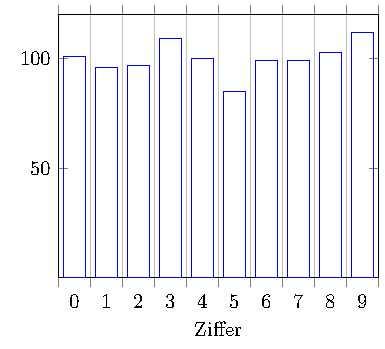
\includegraphics{medien2/basis10/basis10.pdf}
  \centering
  \caption{Ziffernverteilung von $e$ in der basis 10}
\end{figure}
\newpage
\par In dem Graphen ist die Verteilung von Ziffern der ersten 1.000 Stellen von $e$ zu sehen. Zu beachten ist, dass die Ziffer 5 mit 85 mal in dem Abschnitt am Wenigsten vorkommt und die Ziffer 9 mit 112 Mal am Meisten, aber insgesammt erkennt man, dass alle Ziffern relativ gleich Verteilt sind.
\subsubsection{Basis 2}
\begin{figure}[h]
  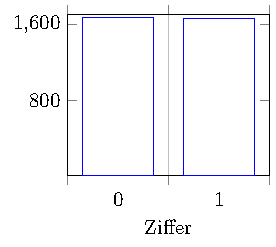
\includegraphics{medien2/basis2/basis2.pdf}
  \centering
  \caption{Ziffernverteilung von $e$ in der basis 2}
\end{figure}
In der Basis 2 ist das gleiche erkennbar. Ziffer 1 und 0 kommen ungefähr gleich oft vor. 
Zahlen, deren Ziffern in einer Basis gleich verteilt sind, nennt man normal. $e$ ist absolut normal, da sie eine normale Zahl in jeder natürlichen Base $>= 2$ ist. Die Zahl $0.\overline{1234567890}$ z.B ist nur normal in Basis 10. Interessant ist, dass es zwar unendlich viele normale Zahlen wie $e$ gibt, aber diese 0\% der Reellen Zahlen ausmachen - genau so wie die rationalen Zahlen.
\subsection{Die Eulersche Zahl als unendlicher Kettenbruch}
Ganz am Anfang wurde der einfache Kettenbruch von $e$ bereits angesprochen (siehe 3.1). Kettenbrüche sind mit dem Euklidischen Algorithmus (ein Algorithmus zum Berechnen des größten gemeinsamen Teilers von 2 Zahlen) eng verbunden. Der Zusammenhang besteht darin, dass der euklidische Algorithmus und Kettenbrüche auf dem Prinzip der fortgeschrittenen Division basieren. Bei Kettenbrüchen kann man die Division als eine Art euklidischen Algorithmus betrachten. Tatsächlich wird der Euklidische Algorithmus dazu verwendet, die Koeffizienten in der Kettenbruchentwicklung einer rationalen Zahl zu finden. Andere interessante Kettenbrüche gehören zu dem Goldenen Schnitt und $\pi$: 
\subsubsection{Andere Kettenbrüche}
\[\phi = [1; 1, 1, 1, \dots]
\]\[\pi =[3; 7, 15 , 1, 292, 1, 1, 1, 2,\dots]
\]Wenn man die ersten 4 Terme des Kettenbruchs von $\pi$ zu einem Bruch vereinfacht, dann erhält man $\frac{355}{113}$ - die beste Fraktionale Näherung von $\pi$, die noch einen relativ kleinen Nenner und Divisor besitzt. Das liegt daran, dass der nächste Term eine große Zahl ist und den Bruch damit komplizierter macht - in anderen Worten: Große Zahl im Kettenbruch bedeutet die Vorherigen Elemente ergeben eine Gute Näherung für eine irrationale Zahl. Deswegen sind die Näherungen aus wenigen Elementen von $\phi$ (welche übringens aus Fibonacci-Zahlen bestehen) auch eher ungenau.
\subsubsection{Auswertung als Näherung von $e$}
Der Graph zur Genauigkeit dieser Näherungsmethode sieht ähnlich aus wie der Graph zur Genauigkeit der Summe (siehe 4.1.1 / Abbildung 2): in beiden scheint der Graph linear zu wachsen, aber der Graph in Abbildung 6 wächst rund 25\% langsamer, aber die x-Achse in Abbildung 2 zeigt die Anzahl an Summanden, während die x-Achse in Abbildung 6 die Anzahl an Elementen des einfachen Kettenbruchs wiedergibt - also ist der Vergleich nicht ganz eindeutig, da aber beide Berechnungen eine Division pro x benötigen, müssten sie in Effizienz vergleichbar sein.
\begin{figure}[h]
  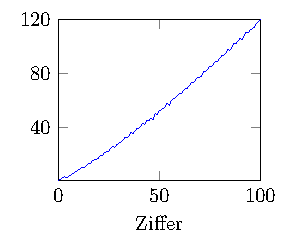
\includegraphics{medien2/kettenbruch/kettenbruch.pdf}
  \centering
\caption{Genauigkeit von $e$ als einfacher Kettenbruch}
\end{figure}
\newpage
